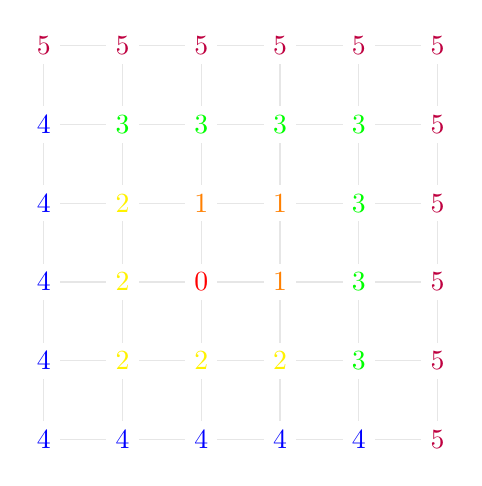
\begin{tikzpicture}
  \draw[step=1.0,gray, opacity=0.2,thin] (-2,-2) grid (3,3);
  
  \draw[color=red] (0,0) node[fill=white] {0};

  \foreach \i in {0, 1} {
    \draw[color=orange] (\i,1) node [fill=white] {1};
    \draw[color=orange] (1,\i) node [fill=white] {1};
  }

  \foreach \i in {-1, 0, 1} {
    \draw[color=yellow] (\i,-1) node [fill=white] {2};
    \draw[color=yellow] (-1,\i) node [fill=white] {2};
  }

  \foreach \i in {-1, 0, 1, 2} {
    \draw[color=green] (\i,2) node [fill=white] {3};
    \draw[color=green] (2,\i) node [fill=white] {3};
  }

  \foreach \i in {-2, -1, 0, 1, 2} {
    \draw[color=blue] (\i,-2) node [fill=white] {4};
    \draw[color=blue] (-2,\i) node [fill=white] {4};
  }

  \foreach \i in {-2, -1, 0, 1, 2, 3} {
    \draw[color=purple] (\i,3) node [fill=white] {5};
    \draw[color=purple] (3,\i) node [fill=white] {5};
  }
\end{tikzpicture}
